\chapter{In-Field Monitoring with Automated IJTAG Instrumentation}
\label{ch:ijtag}

Structural redundancy keeps the accelerator \emph{correct} in the presence of
faults; it does not, on its own, make the accelerator \emph{observable}. For
in-field health management --- tracking temperature, activity, and degradation
over the service life, and reacting before a marginal condition becomes a failure
--- the design must expose internal state through a standard, retargetable
access mechanism. This chapter presents the second framework of the thesis: an
automated flow that inserts IEEE~1687 (IJTAG) sensors into the accelerator's
VHDL hierarchy and builds the on-chip access network around them.

Section~\ref{sec:ij-goal} states the goal and the manual-effort problem it
solves. Section~\ref{sec:ij-sensor} describes the sensor instrument.
Section~\ref{sec:ij-tool} describes the insertion tool and its
configuration. Section~\ref{sec:ij-flow} describes the two-phase Tessent flow
that builds the network. Section~\ref{sec:ij-synth} reports the synthesis cost of
the instrumentation.

\section{Goal: observability without manual rewiring}
\label{sec:ij-goal}

Attaching even a single instrument to an IJTAG network by hand is tedious and
error-prone: the instrument must be declared, instantiated at the right point in
the hierarchy, connected to the scan path with the correct client-interface
signals, described in ICL so that the tool can retarget access to it, and hosted
behind a Segment Insertion Bit (SIB) so it can be switched in and out of the
active chain. Doing this for several instruments scattered across a deep
hierarchy --- and redoing it every time the design changes --- quickly becomes
unmanageable.

The flow developed here removes the manual effort entirely. The designer marks
\emph{where} sensors should go using lightweight pragmas in the VHDL and
\emph{describes} the sensors and their connections once in a JSON configuration
file. A Python tool then performs the mechanical work --- filling in
declarations and instantiations, producing modified source files --- and emits
the Tessent scripts that extract the connectivity and synthesise the IJTAG
network automatically.

\section{The sensor instrument}
\label{sec:ij-sensor}

The instrument used in this work is an \emph{activity sensor}: a small monitor
that counts rising-edge toggle events on a chosen internal signal over a window
and exposes the count, together with an \texttt{alert} bit, through a proper
IJTAG Test Data Register (TDR). Conceptually the same wrapper accommodates other
sensor types --- a thermal monitor, for instance --- since all that the network
sees is a standard 1687 client interface.

The instrument has two clearly separated parts, illustrated in
Figure~\ref{fig:sensor}:

\begin{itemize}
  \item A \textbf{functional side}, clocked by the design clock, which observes
        the monitored signal and maintains the activity counter and alert.
  \item An \textbf{IJTAG client side}, clocked by the scan clock \texttt{tck},
        comprising the TDR and the standard 1687 control signals
        (\texttt{reset}, \texttt{sel}, \texttt{ce}, \texttt{se}, \texttt{si},
        \texttt{so}). At capture time the TDR samples \{\texttt{alert},
        \texttt{activity\_count}\}; the value is then shifted out through the
        network.
\end{itemize}

\begin{figure}[htbp]
\centering
\begin{tikzpicture}[
  box/.style={draw, rounded corners, minimum height=8mm, align=center, font=\footnotesize, fill=blue!6},
  arr/.style={-{Latex[length=2mm]}, thick}]
\node[box, fill=orange!12] (cnt) {Toggle counter\\(\texttt{clk} domain)};
\node[box, right=22mm of cnt] (tdr) {IJTAG TDR\\(\texttt{tck} domain)};
\node[left=10mm of cnt, font=\footnotesize, align=center] (sig) {monitored\\signal};
\node[above=7mm of cnt, font=\footnotesize] (clk) {\texttt{clk}};
\node[right=16mm of tdr, font=\footnotesize] (so) {\texttt{so} (scan out)};
\node[left=6mm of tdr, yshift=-11mm, font=\footnotesize] (si) {\texttt{si, sel, ce, se, tck, reset}};
\draw[arr] (sig) -- (cnt);
\draw[arr] (clk) -- (cnt);
\draw[arr] (cnt) -- node[above, font=\scriptsize] {capture} (tdr);
\draw[arr] (tdr) -- (so);
\draw[arr] (si) -| (tdr.south);
\end{tikzpicture}
\caption{Activity-sensor instrument. The functional counter is sampled into an
IEEE~1687 Test Data Register, which is accessed serially through the standard
client interface driven by the IJTAG network.}
\label{fig:sensor}
\end{figure}

A deliberate design choice is that every IJTAG \emph{input} of the instrument
carries a default value in its port declaration. This allows the instance to be
left with open associations in plain RTL --- the functional simulation and the
Design Compiler elaboration both accept it --- while Tessent connects the client
interface when it inserts the scan network. The instrument is thus valid both
before and after network insertion, which is what makes a clean,
synthesise-anywhere flow possible.

\section{The sensor-insertion tool}
\label{sec:ij-tool}

\subsection{Pragma-marked injection points}

The designer indicates where a sensor's declaration and instantiation should
appear by placing pragma comments in the relevant VHDL files. The tool scans the
hierarchy for these pragmas and replaces them with the concrete declaration and
instantiation generated from the configuration. Because the markers are
comments, an un-instrumented build is completely unaffected.

\subsection{JSON configuration}

A single \texttt{config.json} file describes everything the tool needs: the
top-level entity and working directory, the clock port and period, the cell
libraries and packages, the list of sensor types and their ICL port names, and
--- crucially --- the set of \emph{instances} to create. Each instance names the
sensor type, the generic map (sensor identifier and counter-window width), the
port map binding the instrument's functional ports to real design signals, and
the hierarchical \texttt{tessent\_path} at which the instrument lives.

In this study three activity-sensor instances are defined at three different
levels of the hierarchy, demonstrating that the flow works at arbitrary depth:

\begin{enumerate}
  \item \texttt{act\_sensor\_top} --- at the top level
        (\texttt{/RTL\_DSP\_TOP}), monitoring the accelerator busy signal.
  \item \texttt{act\_sensor\_adders} --- one level down, inside
        \texttt{DSP\_Adders}, monitoring the adder enable.
  \item \texttt{act\_sensor\_adders\_sync} --- two levels down, inside the
        adder synchronisation block, monitoring the adder enable vector.
\end{enumerate}

A \texttt{configurations} section then groups these instances into cumulative
build variants --- \texttt{1sensor}, \texttt{2sensor}, and \texttt{3sensor} ---
so that the cost of progressively adding instruments can be measured (see
Section~\ref{sec:ij-synth}). The relationship is summarised in
Table~\ref{tab:sensors}.

\begin{table}[htbp]
\centering
\caption{Sensor instances and the cumulative build configurations. Each
configuration adds one more activity sensor, at a progressively deeper point in
the hierarchy.}
\label{tab:sensors}
\small
\begin{tabular}{llp{6.0cm}}
\toprule
Build & Instances & Deepest instrumentation point \\
\midrule
\texttt{1sensor} & top                          & \texttt{/RTL\_DSP\_TOP} \\
\texttt{2sensor} & top, adders                  & \texttt{/RTL\_DSP\_TOP/DSP\_Adders} \\
\texttt{3sensor} & top, adders, adders\_sync    & \texttt{.../DSP\_Adders\_Sync\_inst} \\
\bottomrule
\end{tabular}
\end{table}

\subsection{What the tool emits}

For a chosen configuration, the tool writes a set of \emph{modified} VHDL files
(originals untouched) with the pragmas filled in, and generates the Tessent
dofiles for the next phase: an ICL-extraction script per sensor and a single
\texttt{inject\_sensors.tcl} insertion script. A companion driver script then
runs the whole flow --- ICL extraction, IJTAG insertion, and Design Compiler
synthesis --- for every configuration found beside it, capturing and scanning
each step's log for errors.

\section{Building the network: the two-phase Tessent flow}
\label{sec:ij-flow}

Constructing the IJTAG network is done in two phases, reflecting how Tessent
consumes instrument descriptions.

\paragraph{Phase 1 --- ICL extraction.} Each sensor's RTL is read and its
Instrument Connectivity Language (ICL) description is extracted, so that the
tool knows the instrument's scan interface and register layout. This produces a
per-sensor ICL module that the insertion phase can reference.

\paragraph{Phase 2 --- IJTAG insertion.} The full design is read in DFT context;
the previously extracted ICL is read back; and Tessent hosts each instrument
behind a Segment Insertion Bit, wiring the client interfaces into a hierarchical
scan path and connecting it to the top-level TAP. The result is a design in which
all sensors are reachable through one standard IJTAG port, and the access network
can be reconfigured (via the SIBs) to include only the instruments of interest.

The flow encodes several hard-won practical details: the cell libraries are read
as Tessent \texttt{tcelllib} files; VHDL-2008 parsing is enabled; the scan clock
is left for the network to drive rather than being constrained as a functional
clock; and the open-by-default IJTAG inputs of the instrument (Section
\ref{sec:ij-sensor}) let the same instrument elaborate cleanly in all tools.
Figure~\ref{fig:ijtag-flow} summarises the end-to-end flow.

\begin{figure}[htbp]
\centering
\begin{tikzpicture}[
  flowbox/.style={draw, rounded corners, text width=2.6cm, align=center,
                  minimum height=11mm, inner sep=3pt, font=\footnotesize, fill=blue!6},
  arr/.style={-{Latex[length=2mm]}, thick}]
\node[flowbox, fill=gray!12] (vhdl) at (0,0)    {Pragma-marked VHDL\\+ \texttt{config.json}};
\node[flowbox]               (inj)  at (4.7,0)   {Python\\sensor injector};
\node[flowbox]               (icl)  at (9.4,0)   {Phase 1:\\ICL extraction};
\node[flowbox]               (ins)  at (9.4,-2.4) {Phase 2: IJTAG\\insertion (SIBs)};
\node[flowbox]               (dc)   at (4.7,-2.4) {Design Compiler\\synthesis};
\node[flowbox, fill=orange!12] (rep) at (0,-2.4)  {Area / power\\reports};
\draw[arr] (vhdl) -- (inj);
\draw[arr] (inj) -- (icl);
\draw[arr] (icl) -- (ins);
\draw[arr] (ins) -- (dc);
\draw[arr] (dc) -- (rep);
\end{tikzpicture}
\caption{End-to-end automated IJTAG instrumentation flow, from pragma-marked
VHDL to synthesis reports. The injector also emits the synthesis scripts that
drive the final Design Compiler step.}
\label{fig:ijtag-flow}
\end{figure}

\section{Synthesis cost of the instrumentation}
\label{sec:ij-synth}

To quantify the hardware cost of observability, each instrumented configuration
(\texttt{1sensor}, \texttt{2sensor}, \texttt{3sensor}) was synthesised at all
three technology nodes in two accounting modes: \emph{black box}, in which the
sensor instruments are treated as empty boxes, and \emph{counted}, in which they
are synthesised and their cells counted. The difference between the two is the
synthesised cost of the sensor logic plus the IJTAG access-network glue. The
results are collected in Table~\ref{tab:ijtag} and plotted in
Figure~\ref{fig:ijtag-cost}.

\begin{table}[htbp]
\centering
\caption{Area cost of the IEEE~1687 sensor instrumentation. \emph{Counted} synthesises the sensor instruments fully; \emph{black box} treats them as empty. Their difference is the synthesised cost of the sensors plus the IJTAG access network. The cost is about 1.7\% at the mature node and falls within synthesis optimisation noise at the finer nodes.}
\label{tab:ijtag}
\small
\begin{tabular}{llrrr}
\toprule
Node & Sensors & Counted area & Black-box area & Instrument cost (\%) \\
\midrule
IHP 130\,nm & 1 & 1,029,222 & 1,012,067 & +1.70 \\
 & 2 & 1,029,242 & 1,012,127 & +1.69 \\
 & 3 & 1,023,080 & 1,012,067 & +1.09 \\
\midrule
NanGate 45\,nm & 1 & 83,981 & 84,401 & -0.50 \\
 & 2 & 84,127 & 84,569 & -0.52 \\
 & 3 & 84,127 & 85,071 & -1.11 \\
\midrule
NanGate 15\,nm & 1 & 21,764 & 21,809 & -0.21 \\
 & 2 & 21,764 & 21,852 & -0.40 \\
 & 3 & 21,764 & 21,979 & -0.98 \\
\bottomrule
\end{tabular}
\end{table}


\begin{figure}[htbp]
\centering
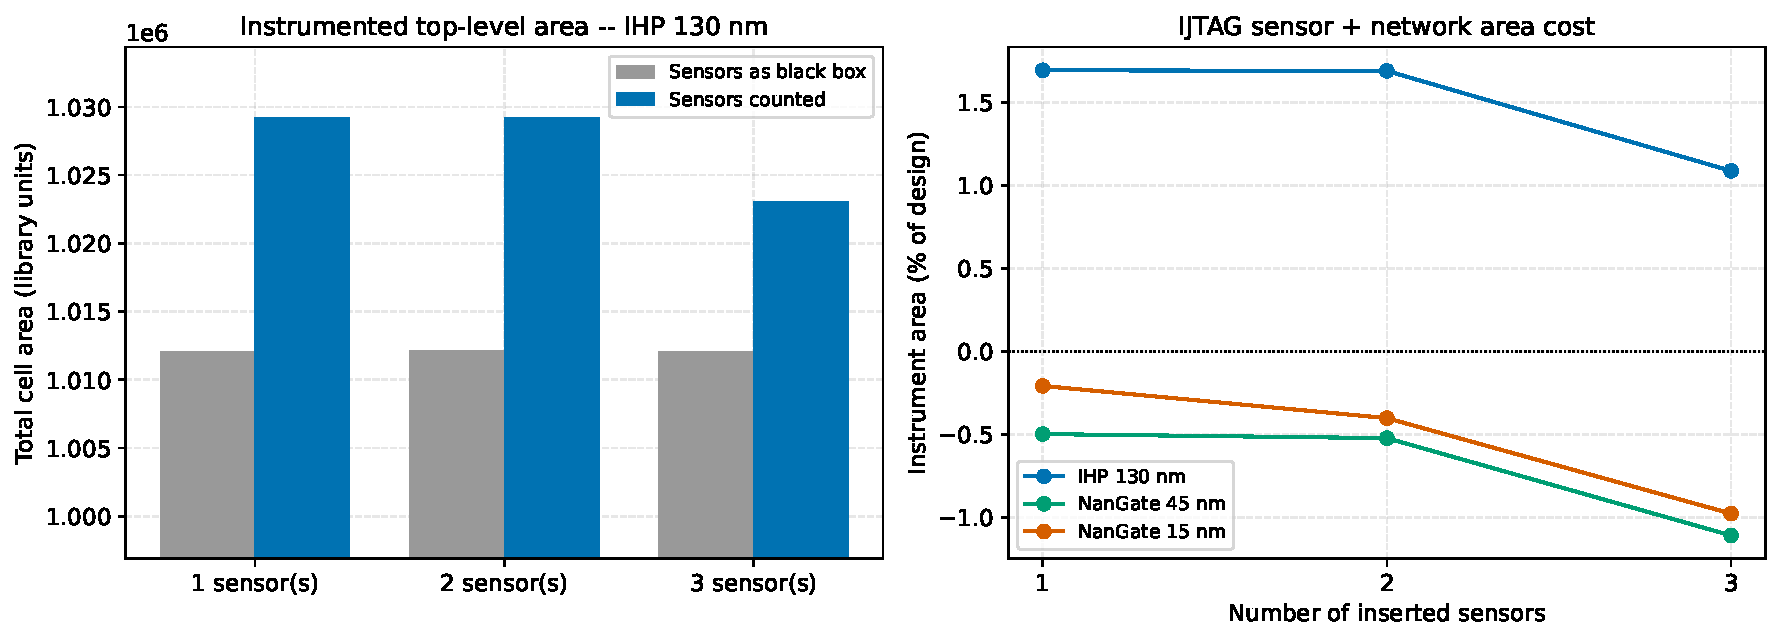
\includegraphics[width=\textwidth]{img/plots/ijtag_cost.pdf}
\caption{Area cost of the IJTAG sensor instrumentation. Left: counted versus
black-box top-level area at the mature node, where the sensor logic is visible
as a small increment. Right: the instrument cost as a percentage of the design,
versus the number of inserted sensors, for the three nodes.}
\label{fig:ijtag-cost}
\end{figure}

Two observations follow. First, the absolute cost of the instrumentation is
\emph{small}: at the mature node the sensors plus network amount to roughly
$1.7\%$ of the (replicated) design, and adding further sensors changes this only
marginally, because the per-sensor logic --- an eight-bit counter and a short TDR
--- is tiny next to a multi-lane vector accelerator. Second, at the finer nodes
the measured difference between the counted and black-box builds falls
\emph{within the run-to-run noise} of synthesis optimisation (it is sub-percent
and can even appear slightly negative, when the optimiser happens to share or
restructure logic differently between the two builds). The honest conclusion is
that, on a design of this size, the area cost of IJTAG-based observability is
negligible-to-minor. In-field monitoring can therefore be added essentially
``for free'' relative to the redundancy overheads quantified in
Chapter~\ref{ch:results}, which makes combining the two frameworks on the same
accelerator very attractive.
